\chapter{Imaging Air Cherenkov Telescopes}
\label{cta}


\section{Detection of Air Showers}
% \subsection{Detecting Gamma Rays}
\label{sec:measuring}

Gamma and cosmic rays cannot be 
observed with IACTs directly. Instead one observes the interaction of
the particles in the atmosphere.

If the primary particle's energy is high enough, the resulting 
secondary particles can interact with the atmosphere themselves, thus starting a 
cascade of secondary particles.
Particles that have enough energy, are faster than the local speed of light.
Because some particles carry a charge and the air acts as dielectricum, 
cherenkov light is emitted \cite{WATSON201113}.

Cherenkov photons are collected by the mirror(s) of a telescope
and projected onto a camera system, usually mounted above the mirror.
Figure \ref{fig:iact_mirror_camera} illustrates the measurement of 
an air shower.

\begin{figure}
	\centering
	\captionsetup{width=0.9\linewidth}
	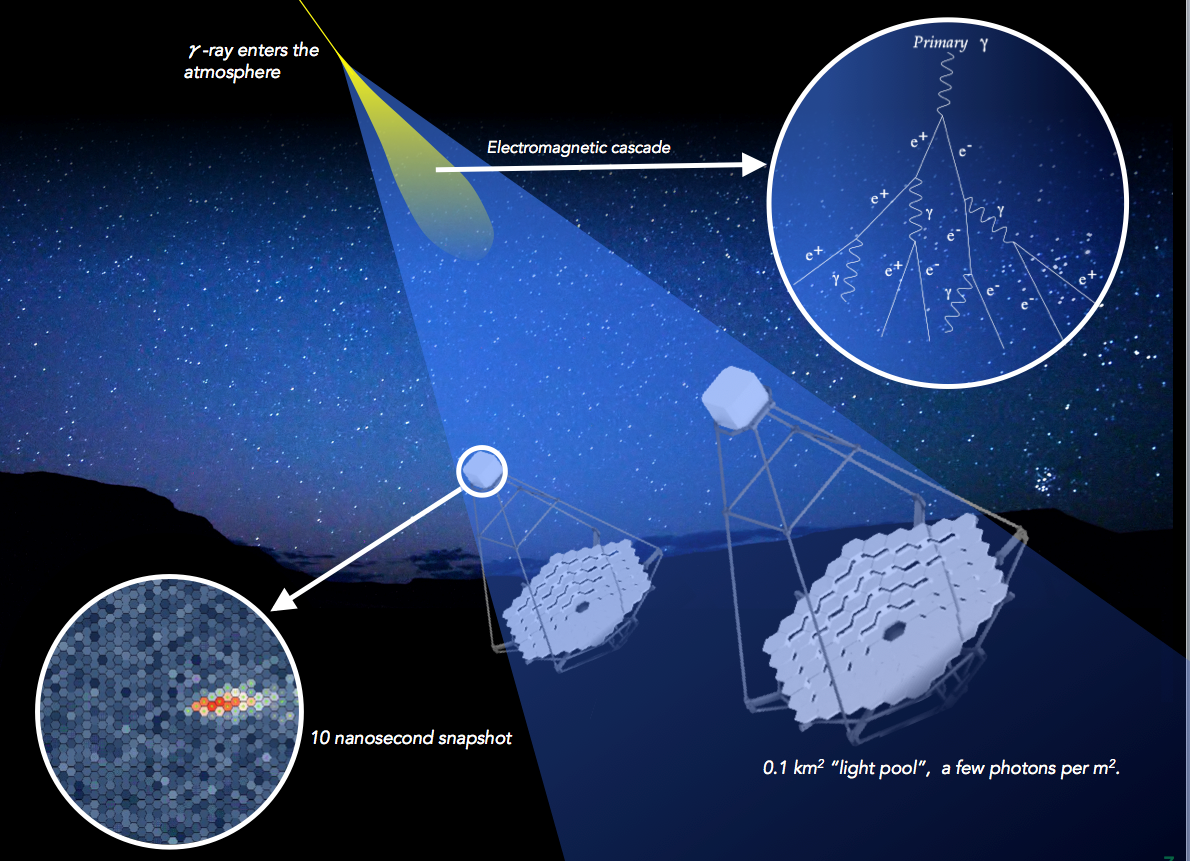
\includegraphics[width=0.8\textwidth]{images/cta47.png}
	\caption{A schematic illustration of the working principles of 
	an IACT experiment:
	Cherenkov light from the air shower 
	hits the mirrors and is focused onto a camera mounted on top.
	An illustration of the resulting image after integrating 
	\SI{10}{\nano\second} of the pixel measurements
	can be seen in the left bottom corner.
	The image is taken from the website 
	of the Cherenkov Telescope Array \cite{cta_web}.}
	\label{fig:iact_mirror_camera}
\end{figure}

Depending on whether the primary particle is 
a photon/electron or a heavier, hadronic particle such as a proton 
or an iron core, the interactions in the atmosphere and the 
produced secondary particles vary.

This leads to a separation of electromagnetic and hadronic showers.
If the experiment is primarily looking for gamma rays,
the hadronic showers act as dominant background.
As hadronic showers are observed much more frequently, 
a good background rejection is crucial to any analysis.

\subsection{Electromagnetic Showers in the Atmosphere}
Electromagnetic showers consist mainly of two types of particles:
\begin{enumerate}
	\item{Photons $\gamma$}
	\item{Electrons e$^-$/Positrons e$^+$}
\end{enumerate}

The main interaction for high energy photons is pair 
production, generating an e$^+$/e$^-$-pair where the summed energy of 
the lepton pair equals the photon energy.
On the other hand, high energy electrons lose 
most of their energy via bremsstrahlung, leading to a new photon
with half the electron's energy.
Only at lower particle energies other interaction forms show their impact,
with scattering and ionization 
leading to more continuous energy losses.

These assumptions lead to the most basic model of an 
electromagnetic shower, proposed by Bhabha and Heitler in 1937
\cite{doi:10.1098/rspa.1937.0082}.
It starts with a high energy primary photon before its interaction in the atmosphere 
and continues the calculation in discrete epochs.
The photon produces a e$^+$/e$^-$-pair in the first epoch.
Because of the high energies at play, the direction of these secondary 
particles does not deviate significantly from the photon's direction, 
making the problem essentially one-dimensional.
The electrons continue on to radiate a photon each and the cycle continues.
Each step doubles the number of particles in the shower with each particle 
on average getting half the energy of its parent particle.
These processes continue until the energies of the particles becomes low enough for
continuous ionization processes to become relevant.
At this point the particle is considered to be stopped and the shower
does not evolve further.

Today, monte carlo calculations are used to simulate the properties 
of particle showers in the atmosphere.
The most commonly used software to model the atmospheric interactions is
CORSIKA \cite{Engel:2018akg}.

Figure \ref{fig:gamma_shower} illustrates the Bhabha-Heitler model (left)
and a \SI{100}{\giga\electronvolt} gamma shower, simulated with CORSIKA (right).

\begin{figure}
	\centering
	\captionsetup{width=0.9\linewidth}
	\begin{subfigure}{.65\textwidth}
  		\centering
  		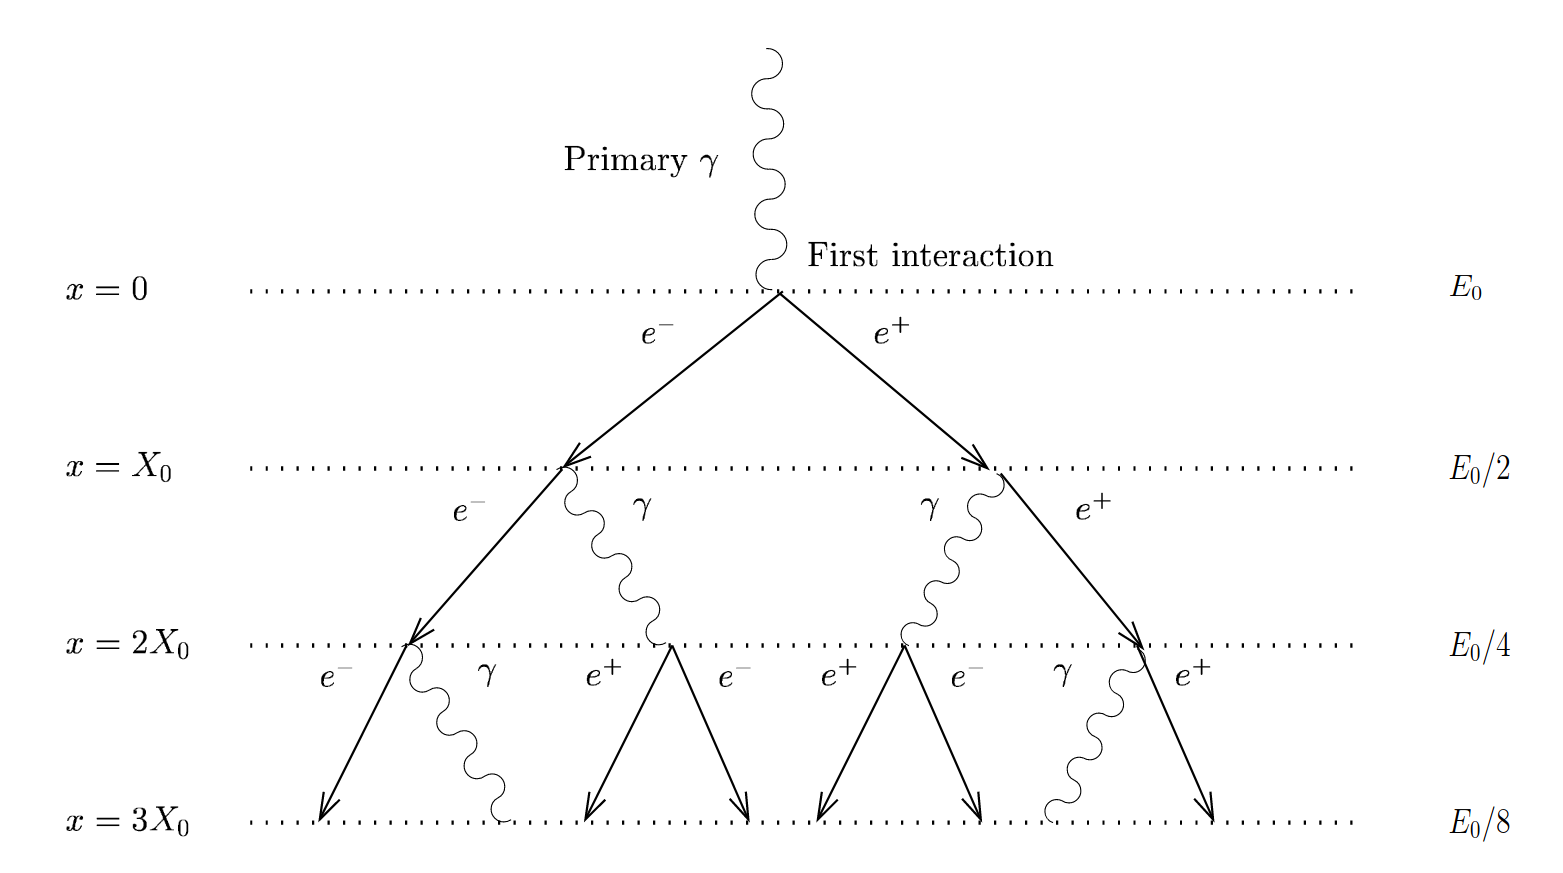
\includegraphics[width=\linewidth]{images/em_shower_illustration.png}
	\end{subfigure}%
	\begin{subfigure}{.15\textwidth}
 		\centering
		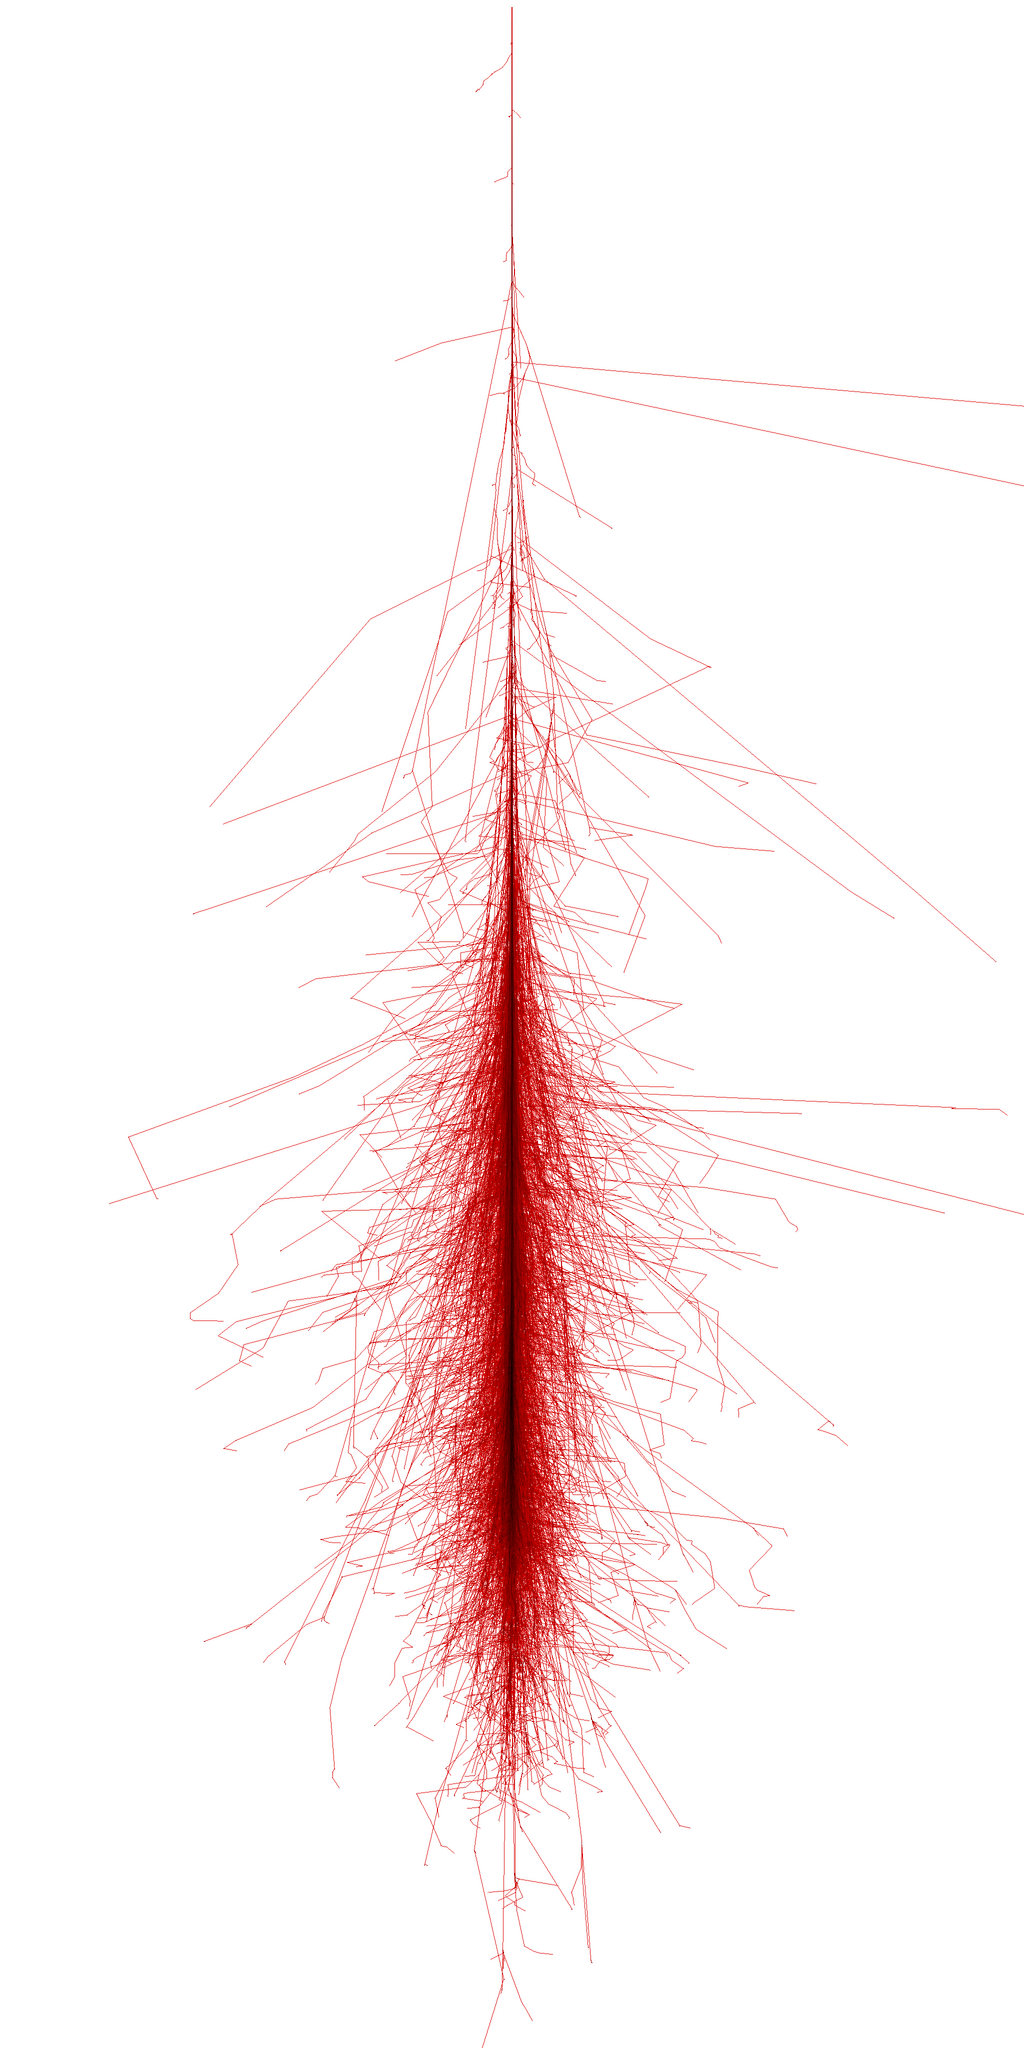
\includegraphics[width=\linewidth]{images/corsika_100gev_photon.png}
	\end{subfigure}
	\caption{
		Left: A schematic illustration of the first epochs of the 
		Bethe-Heitler shower model \cite{funk_doctor}. \\
		Right: A \SI{100}{\giga\electronvolt} gamma-shower as $x$-$z$-projection, simulated with CORSIKA \cite{corsika_showers}.}
	\label{fig:gamma_shower}
\end{figure}

\subsection{Hadronic Showers in the Atmosphere}
Hadronic showers include all the interactions known from 
electromagnetic showers, but add nuclear interactions on top.
These lead to non-negligible additional energy losses 
and the creation of secondary hadronic particles.

Approximations are more difficult to do and monte carlo simulations 
become the only way to reasonably calculate shower behavior.

During the development of the shower, a relevant portion of the particles decay into the 
lightest hadronic particles, pions ($\pi^0, \pi^+, \pi^-$), of which the neutral pions 
rapidly decay into photons.
This means, that part of the hadronic shower
eventually becomes an electromagnetic subshower.

Figure \ref{fig:proton_shower}
shows some of the particles generated in a hadronic shower (left)
and a \SI{100}{\giga\electronvolt} proton shower, simulated with CORSIKA (right).

\begin{figure}
	\centering
	\captionsetup{width=0.9\linewidth}
	\begin{subfigure}{.65\textwidth}
  		\centering
  		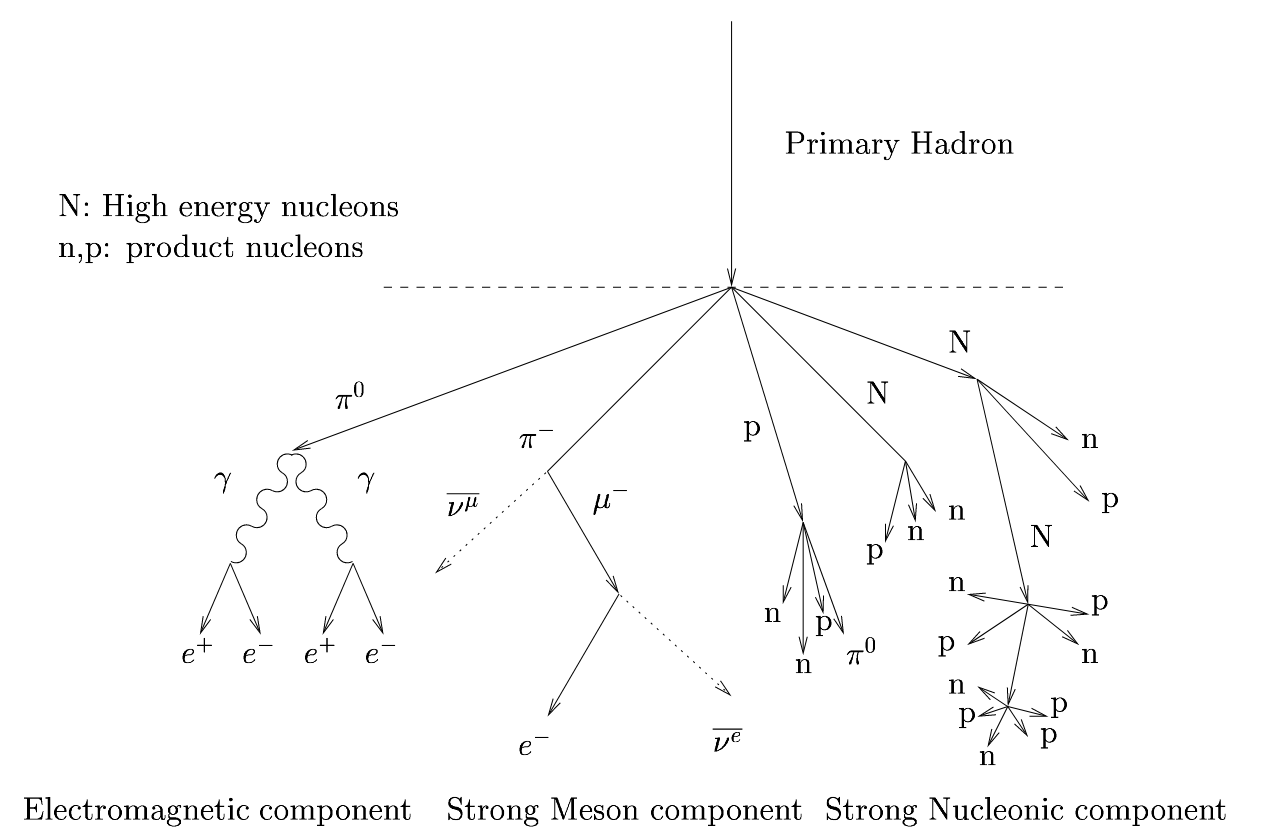
\includegraphics[width=\linewidth]{images/hadron_shower_illustration.png}
	\end{subfigure}%
	\begin{subfigure}{.15\textwidth}
 		\centering
		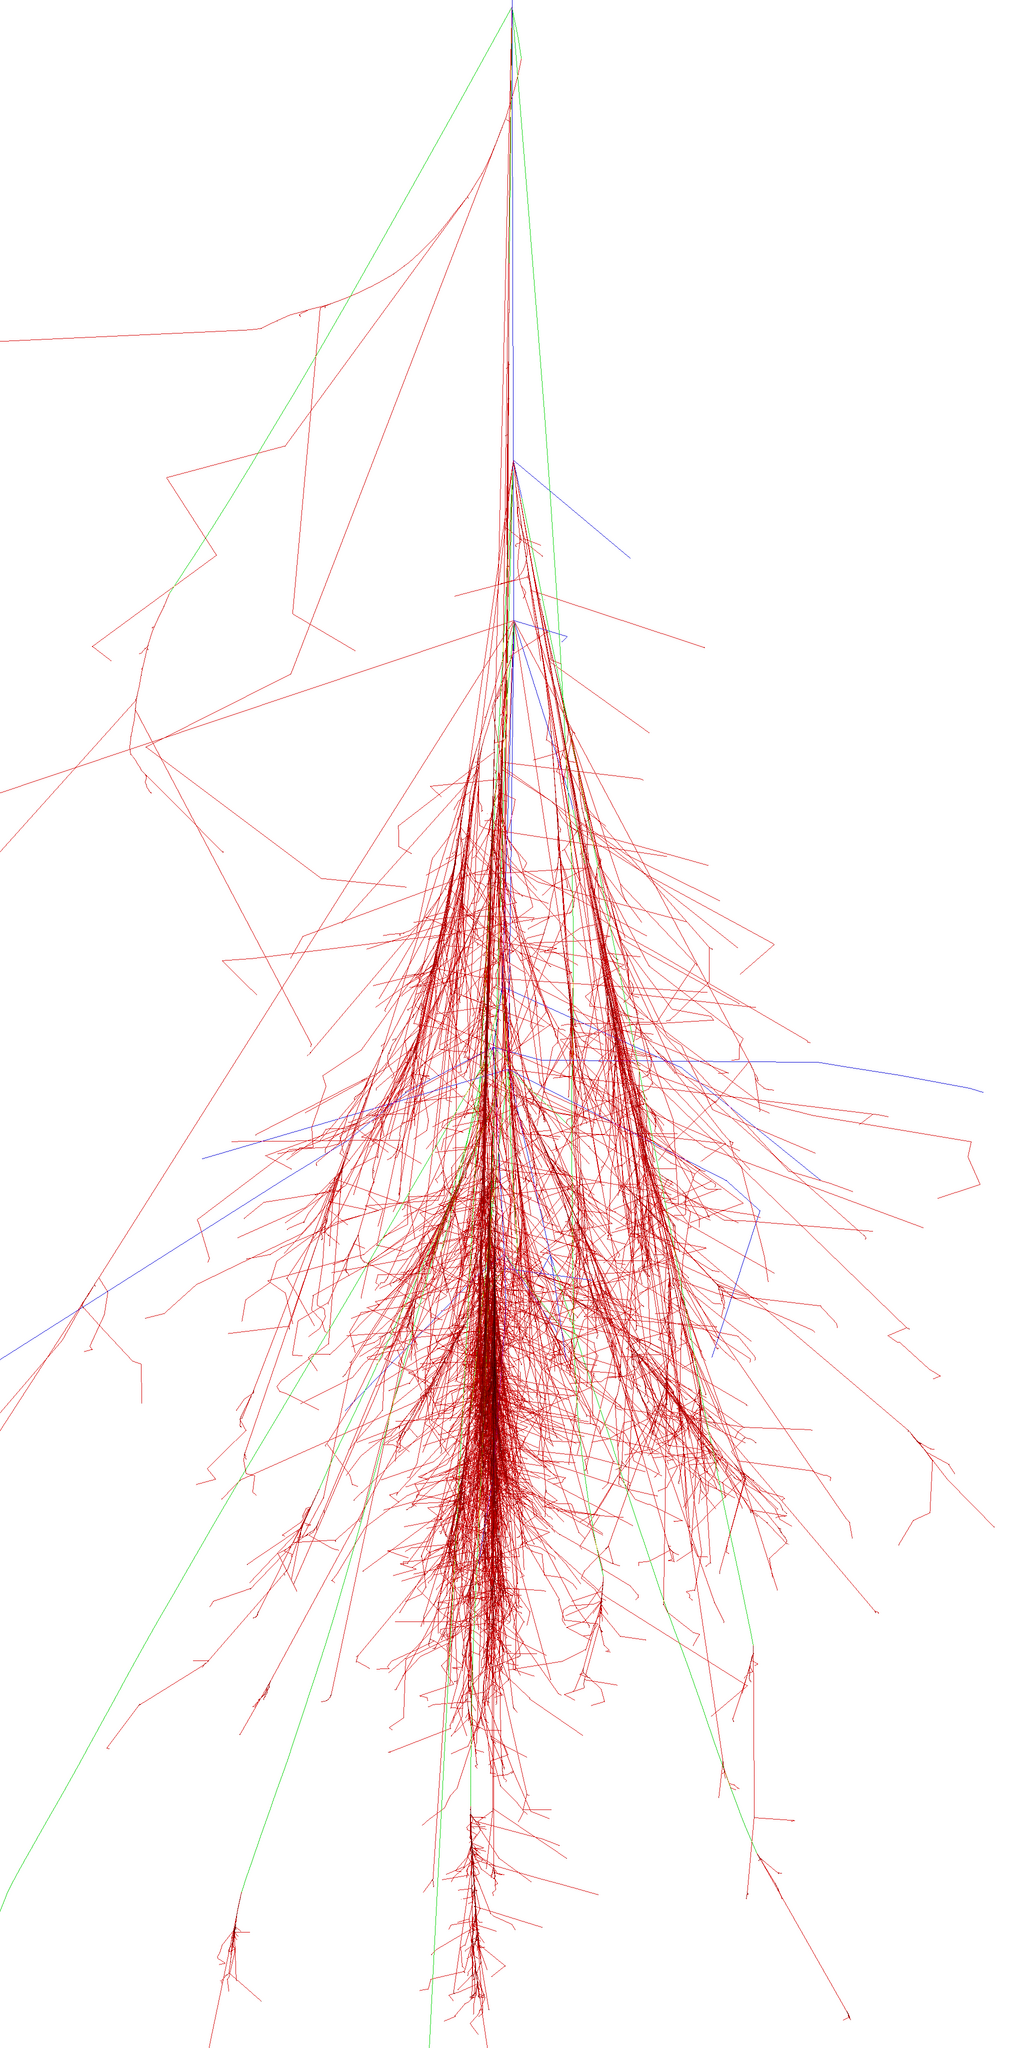
\includegraphics[width=\linewidth]{images/corsika_100gev_proton.png}
	\end{subfigure}
	\caption{
		Left: A schematic illustration of the generation of a hadronic shower \cite{funk_doctor}.\\
		Right: A \SI{100}{\giga\electronvolt} proton-shower as $x$-$z$-projection,
		simulated with CORSIKA \cite{corsika_showers}.}
	\label{fig:proton_shower}
\end{figure}


\section{Current Generation Experiments}

Towards the end of the 1990s, several third generation experiments were
proposed:
H.E.S.S and MAGIC, deriving from parts of the HEGRA collaboration, 
VERITAS from Whipple and the no longer operating CANGAROO from Adelaide and 
several japanese universities \cite{HILLAS201319}. All of these
were designed as stereoscopic imaging telescopes building on the progress made during 
earlier experiments. Two experiments are located on each the northern and the southern hemisphere.

\subsection{Major Atmospheric Gamma Imaging Telescopes (MAGIC)}
MAGIC is a experiment nowadays operating as a stereoscopic setup of two telescopes.
The two telescopes are located at La Palma and have a \SI{17}{\meter} diameter mirror setup each \cite{ALEKSIC201676}.

In the first phase, MAGIC consisted of a single telescope, for differentiation usually
referred to as MAGIC-I. This first phase started 
operation in 2004 and had MAGIC-I be the largest IACT of its time.

The addition of MAGIC-II, the second telescope, in 2009 marked the 
start of the second phase of the experiment and the transition to a third 
generation experiment \cite{2009arXiv0907.1211C}.
In the second phase MAGIC operates in the energy range from \SI{30}{\giga\eV}
up to \SI{100}{\TeV} \cite{magic_website}.

% The DISP-method for the reconstruction of the event arrival direction 
% was significantly improved by including timing information and showed better 
% results for stereoscopy than the simple crossing of the main shower axis \cite{ALEKSIC2012435}.

A specialty of the MAGIC experiment lies in its ability to 
perform fast slews and thus react to gamma-ray bursts, after they have been observed 
by satellite experiments \cite{2003ICRC....5.2943B}.
This enabled the recent observation of the very first \si{\TeV}
gamma-ray burst observed with IACTs \cite{collaboration2019teraelectronvolt}.

The integral sensitivity for a point source is stated to be at
0.67\% of the Crab Nebula Flux, or 0.67\% C.U., above \SI{290}{\giga\electronvolt} 
in 50h of observation time \cite{magic_website}.

\subsection{Very Energetic Radiation Imaging Telescope Array System (VERITAS)}
The VERITAS experiment is located in southern Arizona.
VERITAS	was initially planned as a seven-telescope array, arranged in a diamond shape
and is located in arizona \cite{WEEKES2002221}.

Eventually the collaboration settled 
with four telescopes. 
Each telescope covers a 3.5° FoV with a \SI{12}{\meter} diameter mirror and 
a 499 pixel PMT camera.

A relocation of telescope 1 in 2009 meant that the 
experiment made better use of the given area and its four telescopes,
improving the sensitivity by up to 30\% \cite{2009arXiv0912.3841P}.
% The old and new layout can be seen in figure \ref{fig:veritas_relocation}.

The VERITAS collaboration mentions a lower threshold of \SI{100}{\giga\electronvolt}
with the four telescope setup and a point source sensitivity of
1\% C.U. in 25h \cite{veritas}.

% \begin{figure}
% 	\center
% 	\captionsetup{width=0.9\linewidth}
% 	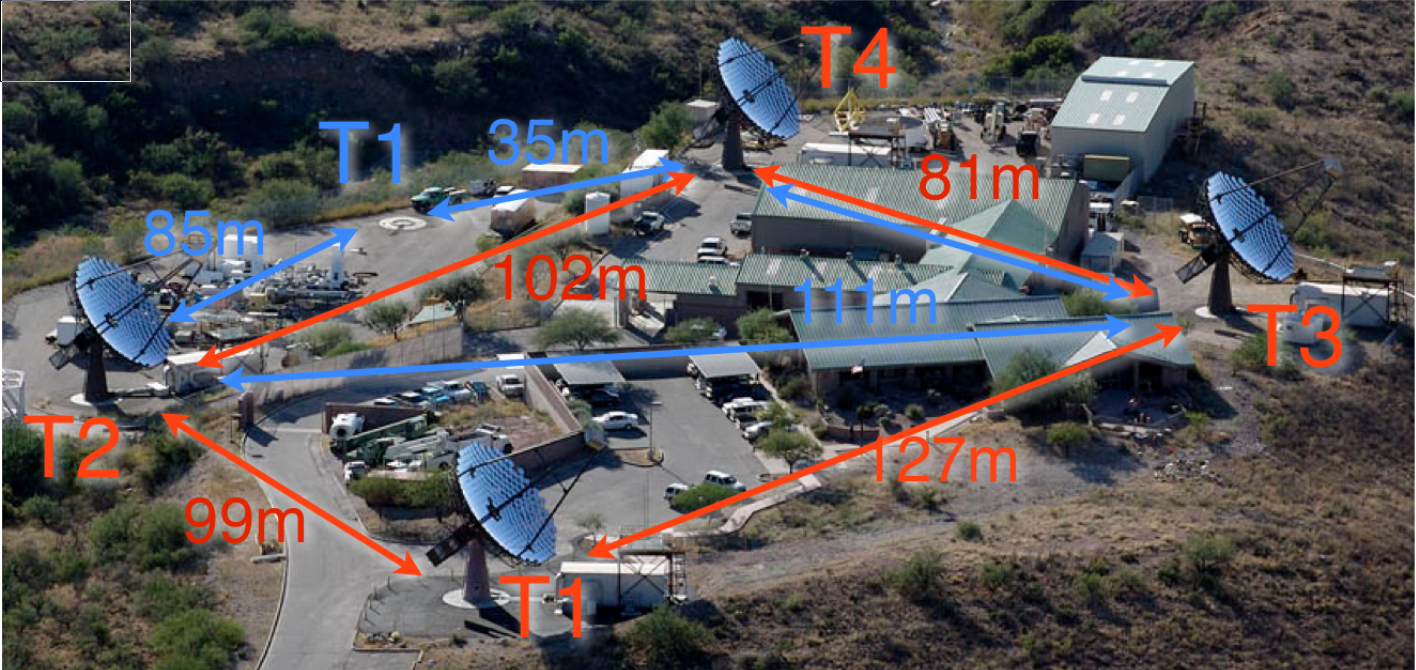
\includegraphics[width=.9\textwidth]{images/veritas_relocation.png}
% 	\caption{The VERITAS array layout after relocation of the first 
% 		telescope. The distances between the telescopes are 
% 		highlighted for the old(blue) and the new(red) array.
% 		In the old setup the telescopes T1, T2 and T4 were too closely
% 		located, making their measurements redundant.
% 	 	The image is taken from an official paper, that investigates
% 		the improved performance gained by relocating the telescope \cite{2009arXiv0912.3841P}.}
% 	\label{fig:veritas_relocation}
% \end{figure}

% Like MAGIC, VERITAS makes use of the DISP-method, especially at large zenith angles 
% \cite{2015ICRC...34..771P}.

\subsection{High Energy Stereoscopic System (HESS)}

The HESS experiment consists of five telescopes and 
is - in contrast to MAGIC and VERITAS - operating in the southern 
Hemisphere, in Namibia.

A similar distinction in phase I and phase II as with MAGIC can be taken with 
HESS phase I consisting of four \SI{13}{\meter} diameter telescopes,
arranged at the edge of a square of \SI{120}{\meter} long sides \cite{HINTON2004331}.
These operated from 2004 to 2012, when the experiment went into phase II.

Phase II brought the larger, fifth telescope with the aim to lower the energy threshold
further. This $\SI{24}{\meter} \times \SI{32}{\meter}$-mirror telescope 
was placed in the middle of the other telescopes.
HESS operates at a similar energy range as MAGIC, stating a lower threshold as low as 
\SI{20}{\giga\electronvolt} \cite{vincent2005hess}.

%SENSITIVITY?\\
%dummy line

\newpage
\section{The Cherenkov Telescope Array}
\label{sec:cta}

The Cherenkov Telescope Array aims to be a next generation IACT experiment.
With two sites of operation, one for each hemisphere, and a number of different 
telescopes proposed, CTA is going to expand on the findings of the third 
generation experiments.

Like HESS in phase II, the CTA arrays are going to consist of differently sized telescopes, namely
the Large-Sized Telescope (LST), 
the Medium-Sized Telescope (MST) 
and the Small-Sized Telescope (SST).
This makes it possible to cover a wide energy range of \SI{20}{\giga\electronvolt}
to \SI{300}{\tera\electronvolt}.

Extensive monte carlo simulations have been performed to find optimal array arrangements
\cite{BERNLOHR2013171}.
The final layouts at La Palma and Chile are shown in figure
\ref{fig:cta_layout}.
The expected sensitivity compared against other currently operating
experiments is shown in figure \ref{fig:cta_performance}.

\begin{figure}[H]
	\center
	\captionsetup{width=0.9\linewidth}
	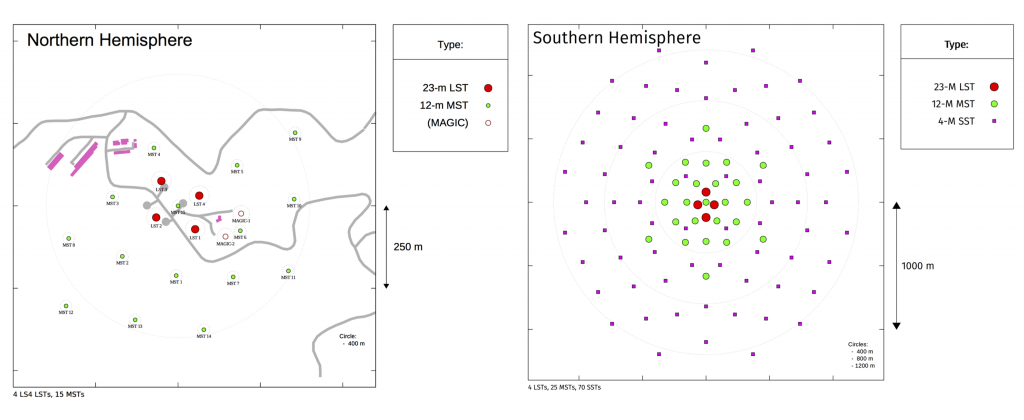
\includegraphics[width=0.9\textwidth]{images/cta_layout.png}
	\caption{
	Left: The array on the northern hemisphere. It will be build at La Palma
	and features only LSTs and MSTs. \\
	Right: The array at the southern hemisphere.
	It will consist of more telescopes and thus 
	work at a wider energy range \cite{cta_web}.}
	\label{fig:cta_layout}
\end{figure}

\begin{figure}[H]
	\center
	\captionsetup{width=0.9\linewidth}
	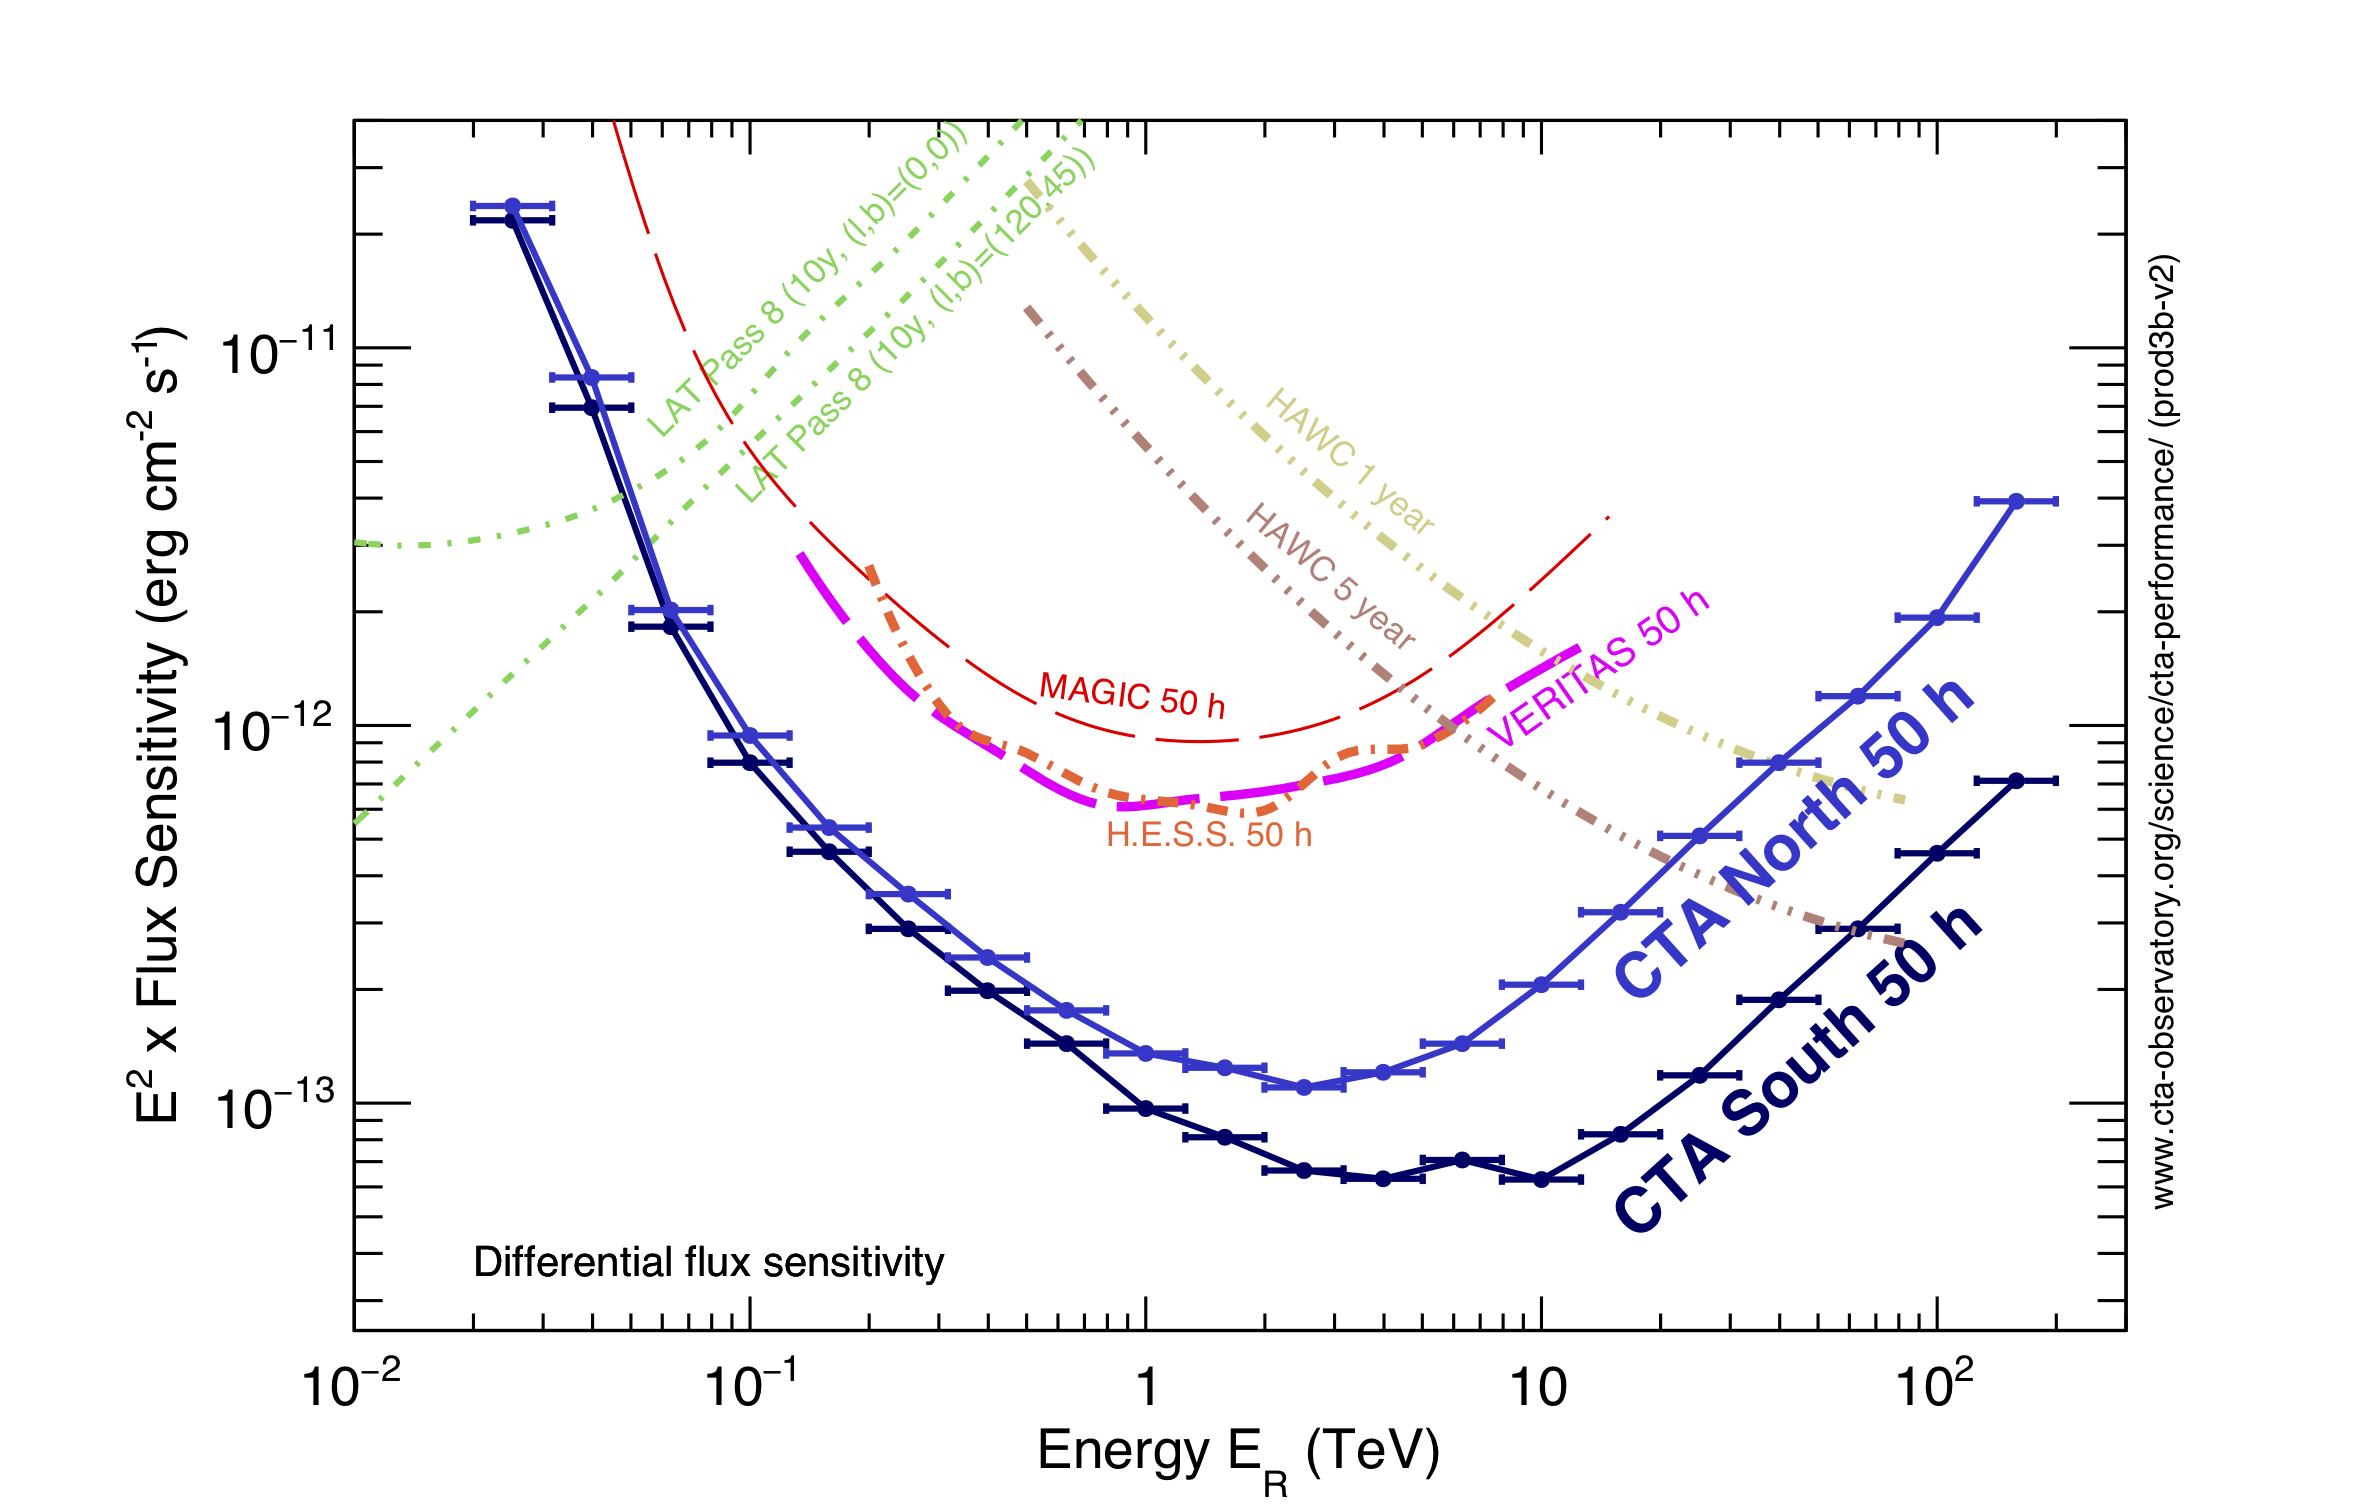
\includegraphics[width=0.9\textwidth]{images/cta_performance.png}
	\caption{A comparison of the expected differential sensitivity of CTA and
	other experiments. The differential sensitivity is defined as the
	minimum flux required to detect a point source with 5$\sigma$ 
	in 50 hours of observation time \cite{cta_web}.}
	\label{fig:cta_performance}
\end{figure}


\subsection{LST}
\label{sec:lst}
The Large-Sized Telescope is going to be biggest telescope of CTA
with a mirror diameter of \SI{23}{\meter}.
It will provide the best sensitivity in the energy range from 
\SI{20}{\giga\electronvolt} to \SI{150}{\giga\electronvolt} with a field of view of \SI{4.3}{\degree}.
The camera of the LST has \num{1855} pixels with two gains each.
The pixels are based on photomultiplier tubes, each seven pixel
form one maintenance module \cite{cta_web}.

The readout electronic is based on the Domino Ring Sampler 
Version 4 chip, which is also used by the MAGIC experiment
\cite{Kubo:2013pwa}. 

Since the LST is looking for the lowest energy gamma rays, it needs
very large mirror areas. At the same time, the effective detector area does 
not need to be as high as for higher energy events.
For this reason, only 4 telescopes are planned per array.

The first LST has been inaugurated at the 10 October 2018 in La Palma \cite{lst_debut}.
It is foreseen to be the first telescope to be operated by the CTA Observatory.
Until then, it has to undergo a critical design review to make sure the performance 
complies with the requirements and expectations.

The telescope is illustrated in figure \ref{fig:lst}.

\begin{figure}
		\centering
		\captionsetup{width=0.9\linewidth}
		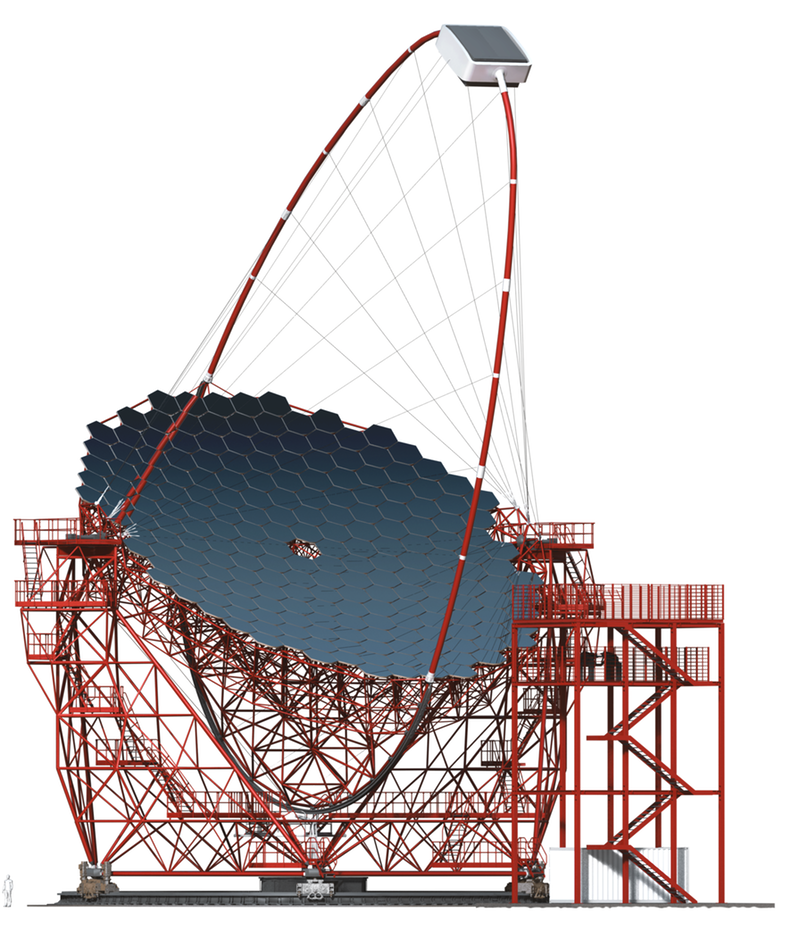
\includegraphics[width=.5\textwidth]{images/LST.png}
		\caption{
			An illustration of the LST with its
			\SI{23}{\meter} diameter parabolic mirror.
			In the lower left corner a human is included for scale \cite{cta_web}.}
		\label{fig:lst}
\end{figure}

%\newpage
\subsection{MST}
The Medium-Sized Telescopes are primarily going to look at the 
energy range from \SI{150}{\giga\electronvolt} to \SI{5}{\tera\electronvolt}.
A total of 15 telescopes on the northern and 25 telescopes on the southern site
will be the backbones of CTA.

Two camera designs are being tested for the MST:
The 1764 pixel FlashCam and the 1855 pixel NectarCam \cite{cta_web}.
The FlashCam combines twelve PMTs to one module and features a completely
digital readout system.
The NectarCam contains an analogue readout chip with a high-gain and a low-gain
channel. 7 PMTs are combined to one module \cite{doi:10.1063/1.4969023}.

A prototype for the MST is standing in Berlin.
It is a fully operational telescope
to validate the component design and assembly processes and is used to test
both cameras.

As an additional approach, a dual mirrored setup, the Schwarzschild-Couder Telescope (SCT), is being tested in arizona \cite{cta_web}.
It features two mirrors with \SI{9.7}{\meter} and \SI{5.4}{\meter} diameter respectively
as well as its own camera system, the SCTCam.
It might be added as complement to the other telescopes.
This silicon photomultiplier based camera includes 11328 pixels and covers a FoV of
\SI{7.6}{\degree}.
The prototype is being tested to gain experience with the optical alignment and operation of
the camera as well as to demonstrate the performance of the setup.

The two setups are illustrated in figure \ref{fig:mst_comp}.

\begin{figure}
    \centering
    \begin{subfigure}[t]{0.35\textwidth}
        \centering
		\captionsetup{width=0.9\linewidth}
		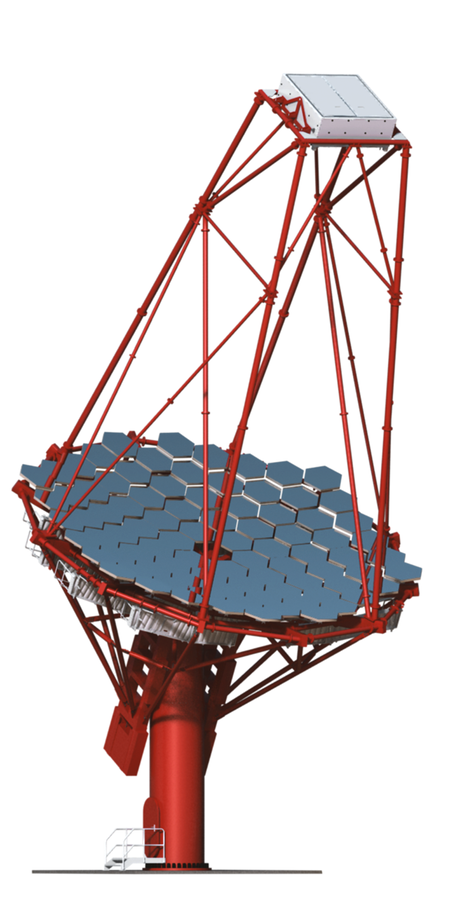
\includegraphics[width=.45\textwidth]{images/MST-1.png}
    \end{subfigure}%
	~
    \begin{subfigure}[t]{0.55\textwidth}
        \centering
		\captionsetup{width=0.9\linewidth}
		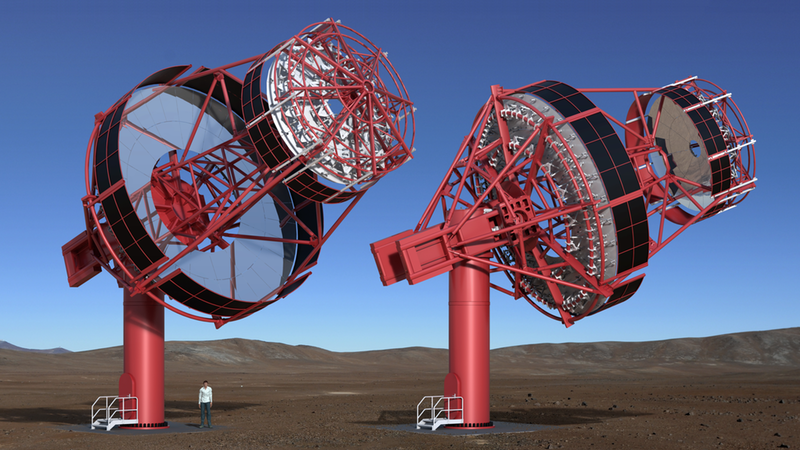
\includegraphics[width=.9\textwidth]{images/SCT.png}
    \end{subfigure}
    \caption{
	Left: An illustration of the MST with its
		\SI{11.5}{\meter} diameter mirror.
		The mirror design is based on the Davies-Cotton design. \\
	Right: An illustration of the SCT with its
		two mirrors. The camera is not included.
		The dual-mirror Schwarzschild-Couder setup includes mirrors of
		\SI{9.7}{\meter} and \SI{5.4}{\meter} diameter \cite{cta_web}.}
	\label{fig:mst_comp}
\end{figure}


%\newpage
\subsection{SST}

The Small-Sized Telescopes (SST) will provide the sensitivity for CTA at the 
highest energies upwards from \SI{5}{\tera\electronvolt}.
An upper limit for the sensitivity is expected to be at around \SI{300}{\tera\electronvolt}.

The design for the SST includes two mirrors, a \SI{4.3}{\meter} and a \SI{1.8}{\meter}
mirror, before the light hits the camera.

In contrast to the LST and MST, the SST's camera includes silicon photo-multipliers
and a total of 2048 pixels. With this the SST is going to cover a field of view 
of \SI{10.5}{\degree}.

The northern array is not going to include any SSTs, the 
southern array on the other hand will contain a total of 70 telescopes over
several square kilometers \cite{cta_web}.

\begin{figure}
		\centering
		\captionsetup{width=0.9\linewidth}
		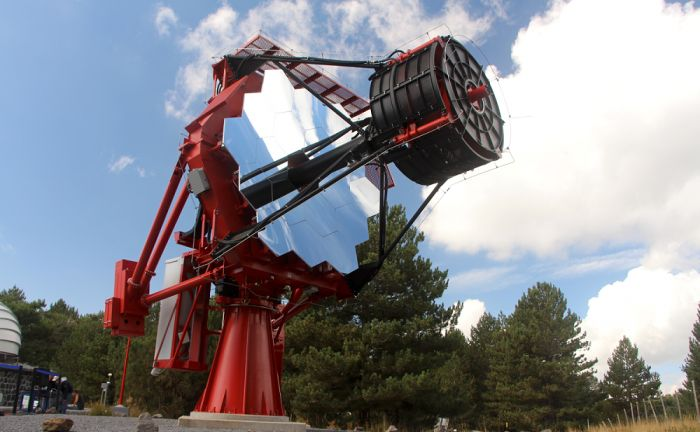
\includegraphics[width=.8\textwidth]{images/sst.jpg}
		\caption{A photo of the ASTRI/CHEC design, that is supposed
		to form the basis of the SST.
		The dual-mirror Schwarzschild-Couder setup includes mirrors of
		\SI{4.3}{\meter} and \SI{1.8}{\meter} diameter \cite{cta_web}.}
		\label{fig:sst}
\end{figure}